
%
%  $Description: Author guidelines and sample document in LaTeX2e$
%
%  $Author: ienne, paulley $
%  $Date: 2002/04/15 11:20:59 $
%  $Revision: 1.0 $
%

\documentclass{ieee}

%-------------------------------------------------------------------------
%
% Use \documentclass[pagenumbers]{ieee}
%
% to produce page numbers, bottom centered, in the output. Default is
% no page numbers for camera-ready copy.
%
%-------------------------------------------------------------------------

\usepackage{times}
\usepackage{listings}
\usepackage[utf8]{inputenc}
\usepackage[brazil]{babel}
\usepackage[T1]{fontenc}
\usepackage{graphicx}
\usepackage{xcolor}
% Definindo novas cores
\definecolor{verde}{rgb}{0,0.5,0}
% Configurando layout para mostrar codigos C++
\usepackage{listings}
\lstset{
  basicstyle=\ttfamily\small,  
  extendedchars=true, 
  showspaces=false, 
  showstringspaces=false, 
  numbers=left,
  numberstyle=\tiny,
  breaklines=true, 
  backgroundcolor=\color{green!10},
  breakautoindent=true, 
  captionpos=b,
  xleftmargin=0pt,
}

\begin{document}


\title{ Experimento 1 - Remasterização de um sistema operacional
Linux embarcado aplicado a um sistema de processamento de imagens
}

\author{André Mateus R. Dantas\\
Matrícula: 11/0008359\\
Universidade de Brasília - Faculdade Gama \\
ymateus@hotmail.com\\
% For a paper whose authors are all at the same institution,
% omit the following lines up until the closing ``}''.
% Additional authors and addresses can be added with ``\and'',
% just like the second author.
}

\maketitle
\thispagestyle{empty}

%-------------------------------------------------------------------------
\section{Objetivos}

Remasterização do Damn Small Linux para uma plataforma embarcada aplicado a um sistema de
processamento de imagens.

%------------------------------------------------------------------------
 \section{Introdução}
Utilizou-se a remasterização para criarmos um sistema embarcado dedicado para criarmos a solução ao
problema protosto.

Este experimento irá  simular um sistema de interceptação (que será simulada por meio de arquivos)
e decodificação de informações esteganografadas em vídeos (sequencia de imagens). A esteganografia é
uma técnica utilizada para esconder uma informação dentro de outra. Observe que seu propósito é
diferente ao da criptografia, onde o objetivo é proteger o conteúdo da mensagem.

%------------------------------------------------------------------------
\section{Especificação dos Sistema }
\subsection{Descrição do sistema implementado}
Uma das formas mais comuns da esteganografia é utilizando a técnica denominada \textit{Least Significant Bits}
(LSB), que consiste em utilizar os bits menos significativos para codificar a mensagem a ser escondida. Que foi a
técnica utilizada nas imagens nesse experimento.Entretanto a esteganografia por LSB é muito vulnerável, pois é
possível detectar e extrair a informação escondida com facilidade utilizando algumas técnicas de esteganálise. 
E portanto, foi inserido ao sistema de esteganografia um processo simples de embaralhamento. Neste caso, a esteganografia foi
implementada em apenas um ou nenhum pixel para cada bloco de tamanho 3x3 pixels da imagem da
seguinte forma:

\begin{center}
\begin{tabular}{|c|l|r|}
\hline
1 & 4 & 7 \\
\hline
2 & 5 & 8\\
\hline
3 & 6 & 9\\
\hline
\end{tabular} 
\end{center}

O valor 0 indica que não existe nenhum pixel que foi esteganografado naquele bloco. Esta posição é
obtida externamente utilizando uma chave decimal de forma circular. E cada bloco é analisado sem que
haja sobreposição entre eles. Já os blocos da borda que não possuírem tamanho 3x3 foram
desconsiderados, ou seja, não possuem informação esteganografada. E por fim deve ser feito um processo de flipagem
nos bits decodificados o que causa um efeito visual melhor.

O sistema irá inserir um cabeçalho à imagem processada. O formato que será utilizado é o
PGM (\textit{portable graymap}), que contém um cabeçalho e a matriz correspondente da imagem. O cabeçalho
pode ser feito inserindo a seguinte informação: P5 W H M I, onde P5 indica o formato PGM, W = largura
em pixels, H = altura em pixels, M = valor máximo do pixel e I = imagem desesteganografada. Neste caso,
o valor dos pixels são representados por um byte, ou seja, variam entre 0 e 255. Neste caso, o cabeçalho será inserido 
na imagem processada por um programa, utilizando a chamada de sistema \textbf{\textit{system()}}.
Uma funcionalidade básica adicionada ao sistema é a capacidade de receber o sinal de interrupção (SIGINT),
que é emitido aos processos do terminal quando as teclas de interrupção (por exemplo: CTRL+c) do teclado são acionadas, 
o código deve abortar o processamento inserindo zeros até o preenchimento dos pixels da imagem processada, em
seguida inserir o cabeçalho à imagem parcialmente processada.

\subsection{Implementação e prototipação}
A solução proposta para o problema apresentado consiste em dois programas (um que desesteganografa a imagem e o outro insere o cabeçalho
a esta imagem). O primeiro programa é basicamente composto pelas funções: aloca\_matriz(int i, int j), colher\_dados(), desembaralha(), flip(), interromper() e a
main(). A função aloca\_matriz simplismente aloca uma matriz com as dimensões i e j. A função colher\_dados apenas lê os dados necessários
do arquivo de parâmentros (parametros.txt).

Já na função desembaralha trabalho sobre a matriz que contém todo o vídeo, percorre essa matriz 
incrementado de 3 em 3 (tanto nas linhas quanto nas colonas), e a partir do valor da chave ele define qual pixel da matriz formada pelos 
valores nos índices:

\[ \left( \begin{array}{ccc}
(i,j) & (i,j+1) & (i,j+2) \\
(i+1,j) & (i+1,j+1) & (i+1,j+2) \\
(i+2,j) & (i+2,j+1) & (i+2,j+2) \end{array} \right)\] 

Como os valores de i e j são incrementados de 3 em 3, temos que todas as imagens do video são varridas em blocos de matrizes 3x3 e de acordo
com a chave o valor correto é selecionado ou nenhum valor é. Isso se repete até que a imagem de saída esteja completa, esta e a função 

flip, que inverte os bits de cada pixel da imagem montada na função desembaralha, são basicamente onde se encontra todo o processamento 
do sistema.

A função interromper(), esta associada a um sinal (SIGINT), que é disparado pelas teclas CTRL+C do teclado, fazendo com que o programa
insira o cabeçalho na imagem processada até ali (os elementos não processados da imagem já terão o valor 0, pois a matriz foi alocada com
o comando malloc, que já aloca a matriz e a preenche com zeros) e encerra o programa. Já na função main copia-se o valor dos elementos do vídeo 
para uma matriz dimanicamente alocada, inicializa-se as duas threads associadas as funções desembaralha e flip e se escreve a imagem resultante.		

Para compilar esse código e execultar o progama basta utilizar as seguintes linhas de comando na pasta onde os arquivos estao:

\begin{flushleft}
\textbf{\$gcc -o cabecalho cabecalho.c}

\textbf{\$gcc -o exp1 exp1.c -lpthread}

\textbf{\$./exp1} 
 
\end{flushleft}



Agora vamos remasterizar o DSL, o primeiro passo é definir um local que será o ambiente de trabalho,
para isso criou-se uma pasta chamada DSL no diretório home.

\begin{flushleft}
\textbf{\# cd /home; mkdir DSL}  
\end{flushleft}




Dentro de DSL baixou-se a distro dsl-4.4.10-embedded.zip, então criou-se duas pastas: a primeita denominada dsl-4.4.10-embedded, 
local onde foi descompactada o arquivo dsl-4.4.10-embedded.zip e a segunda nomeu-se remaster e continha três outros diretórios : 
image, para montar o sistema de arquivos da distro. Master, usada para inserir a nova distro que será gravada no cartão de memória.
E source/KNOPPIX, que foi o diretório fonte da nova distro.

\begin{flushleft}

\textbf{\# cd DSL;
\# mkdir dsl-4.4.10-embedded
\\
\# wget --user=aluno --password=UnB\_Gama http://www.image.unb.br/mintsu/Gama/SistEmb/dsl-4.4.10-embedded.zip aluno UnB\_Gama 
\\
\# unzip dsl-4.4.10-embedded.zip -d dsl-4.4.10-embedded
\\
\# rm dsl-4.4.10-embedded.zip
\\
\# mkdir remaster; cd remaster
\\
\# mkdir -p image master source/KNOPPIX
} 
\end{flushleft}

Em seguida copiou-se  a distribuição dsl-4.4.10-embedded para o diretório master.

\begin{flushleft}
 \textbf{\# rsync -Hav ../dsl-4.4.10-embedded/. master}
\end{flushleft}

Então fez-se a descompressão do KNOPPIX na forma de um arquivo temporário tmp.iso, para isso instalou-se o pacote cloop-utils. 
\begin{flushleft}
 \textbf{\# apt-get install cloop-utils\\
 \#touch tmp.iso\\
 \# extract\_compressed\_fs master/KNOPPIX/KNOPPIX tmp.iso \\
 }
\end{flushleft}

O próximo passo foi montar o arquivo tmp.iso em image, e copiou-se o conteúdo para source/KNOPPIX.

\begin{flushleft}
 \textbf{\# mount -o loop tmp.iso image
\# rsync -Hav image/. source/KNOPPIX
\# umount image 
}
\end{flushleft}

Removeu-se então o arquivo tmp.iso e a pasta image.
\begin{flushleft}
 \textbf{\# rm -R image tmp.iso}
\end{flushleft}

Nesse ponto entrou-se no diretório raiz do Damn Small Linux, disponível em source/KNOPPIX. 
Então mudou-se a flag de vdso-enabled para 0, permitindo assim o uso do comando chroot. Em seguida montou-se o diretório proc, com os 
comandos a seguir.
\begin{flushleft}
 \textbf{\# echo 0 > /proc/sys/abi/vsyscall32\\
\# chroot souce/KNOPPIX\\
\# mount -t proc /proc proc \\
}
\end{flushleft}

O passo seguinte foi a inserção de pacotes do Debian, como o Mirror responsável pelos downloads
 de arquivos DSL estava desatualizado foi preciso modificá-lo pelo recente. Então habilitou-se o apt-get e o atualizou.
\begin{flushleft}
 \textbf{\#echo Mirror:\ distro.ibiblio.org/pub/linux/distributions/damnsmall/ >/opt/.dslrc; echo Protocol:\ http >>/opt/.dslrc\\
\# dpkg-restore\\
\# dpkg -l\\
\# apt-get update\\
}
\end{flushleft}

 Enfim, possibilitou-se a instalação do minicom e do gcc para DSL de forma fácil:
\begin{flushleft}
 \textbf{\# apt-get install minicom\\
\#apt-get install gcc\\
}
\end{flushleft}

A partir desse ponto, tem-se o novo Damn Small Linux com os novos recursos, então desmontou-se /proc e saiu-se do chroot.
\begin{flushleft}
 \textbf{\# umount /proc\\
\# exit\\
}
\end{flushleft}

Removeu-se o arquivo KNOPPIX da distro anterior e em seguida criou-se um novo arquivo KNOPPIX.
\begin{flushleft}
 \textbf{\# rm master/KNOPPIX/KNOPPIX\\
\# mkisofs -R -U -V -hide-rr-moved -cache-inodes -no-bak -pad source/KNOPPIX | create\_compressed\_fs - 65536 > master/KNOPPIX/KNOPPIX\\
}
\end{flushleft}

Ápos esse ponto, bastou formatar o pendrive utilizando o Gparted, copiar os arquivos da pasta master para o dispositivo e instalar e torná-lo
bootavel com o syslinux, com os seguintes comandos:
\begin{flushleft}
 \textbf{\# mount -t vfat /dev/sdb1 /mnt/card;
 \# rsync -Hav /home/DSL/remaster/master/. /mnt/card\\
\# syslinux -- install /dev/sdb1\\
\# umount /mnt/card\\}
\end{flushleft}

%-------------------------------------------------------------------------
\section{Resultados e Discussões}

Como resultados deste experimento temos o total de quatro imagens geradas a partir dos arquivos de vídeo propostos.
Duas eram fotos da Lena Söderberg com uma diferença de constraste, a terceira ela de um homem andando com um guarda-chuva
e a terceira, que segue a baixo, todas rodaram no DSL rematerizado.

  \begin{figure}[h]

	\centerline{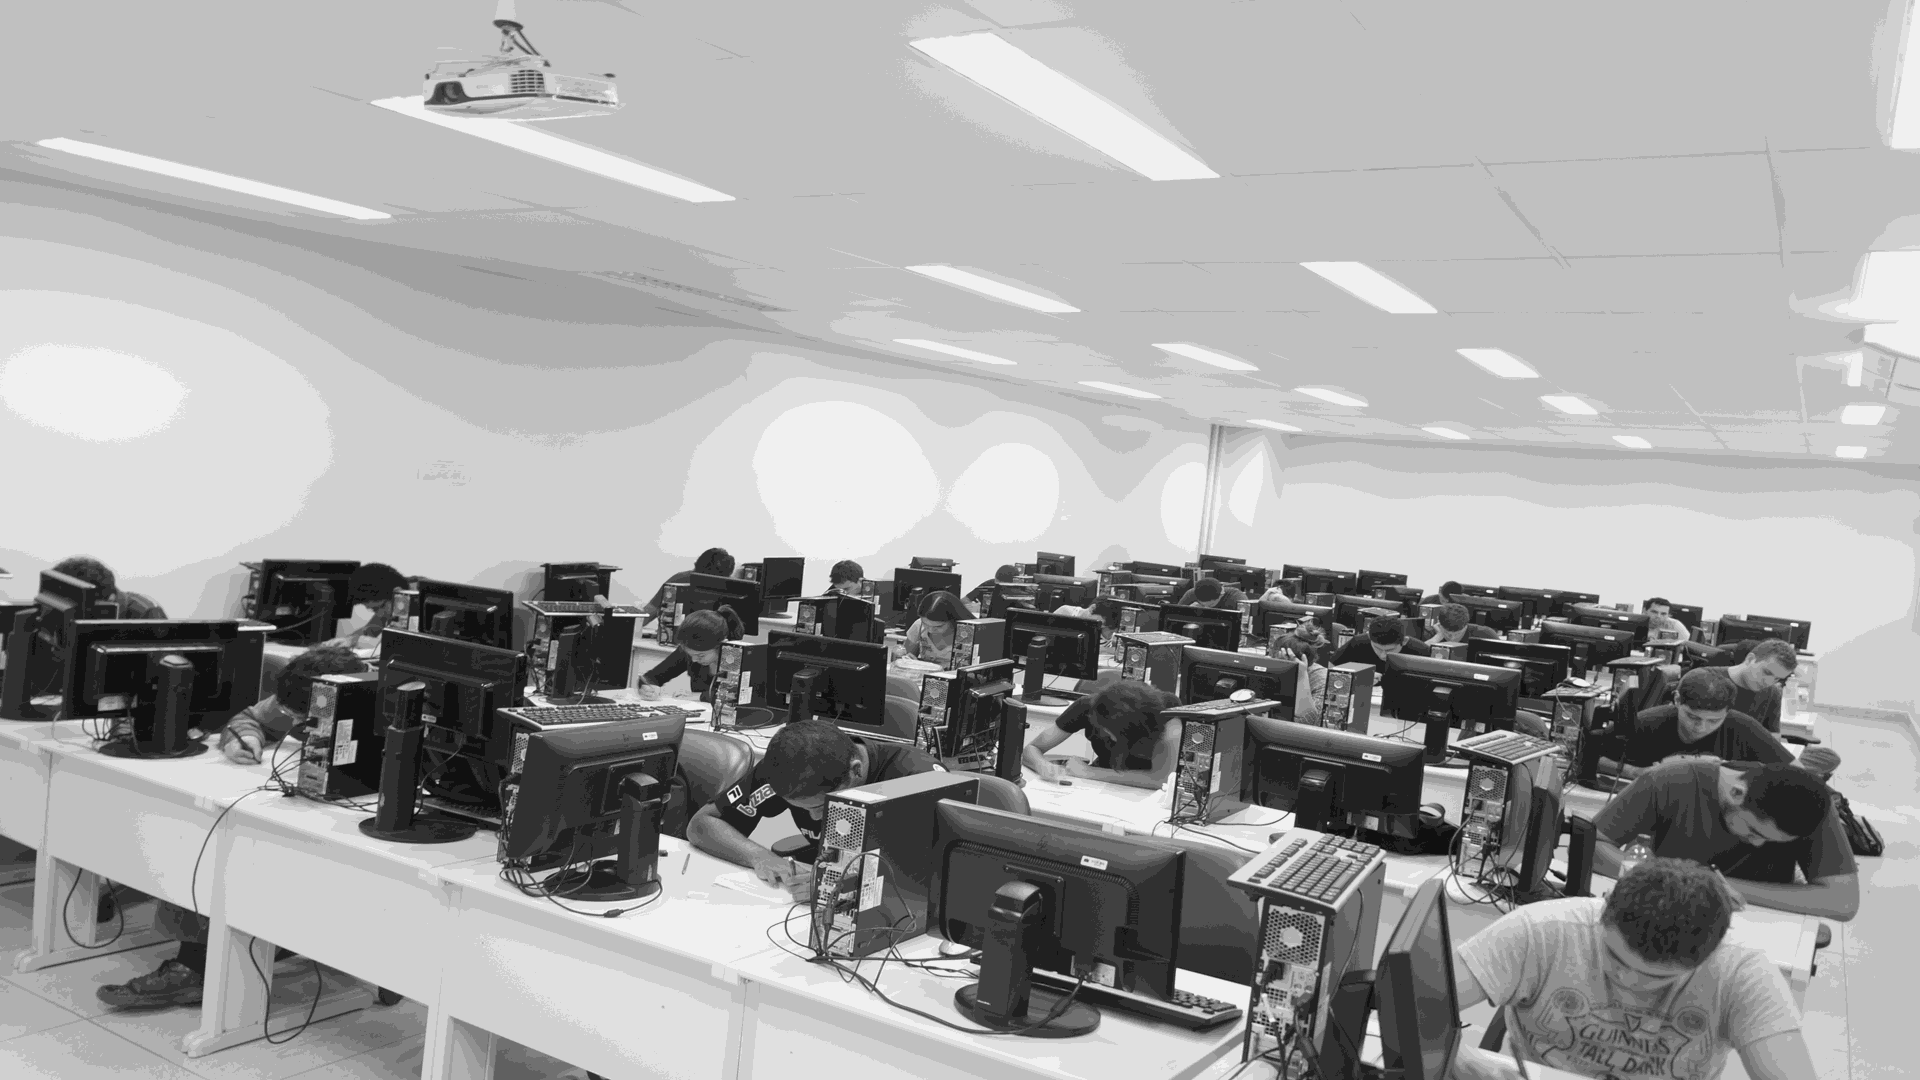
\includegraphics[scale=0.12]{result.png}}	

	\caption{Alunos durante a prova.}

\end{figure}
  \begin{figure}[h]

	\centerline{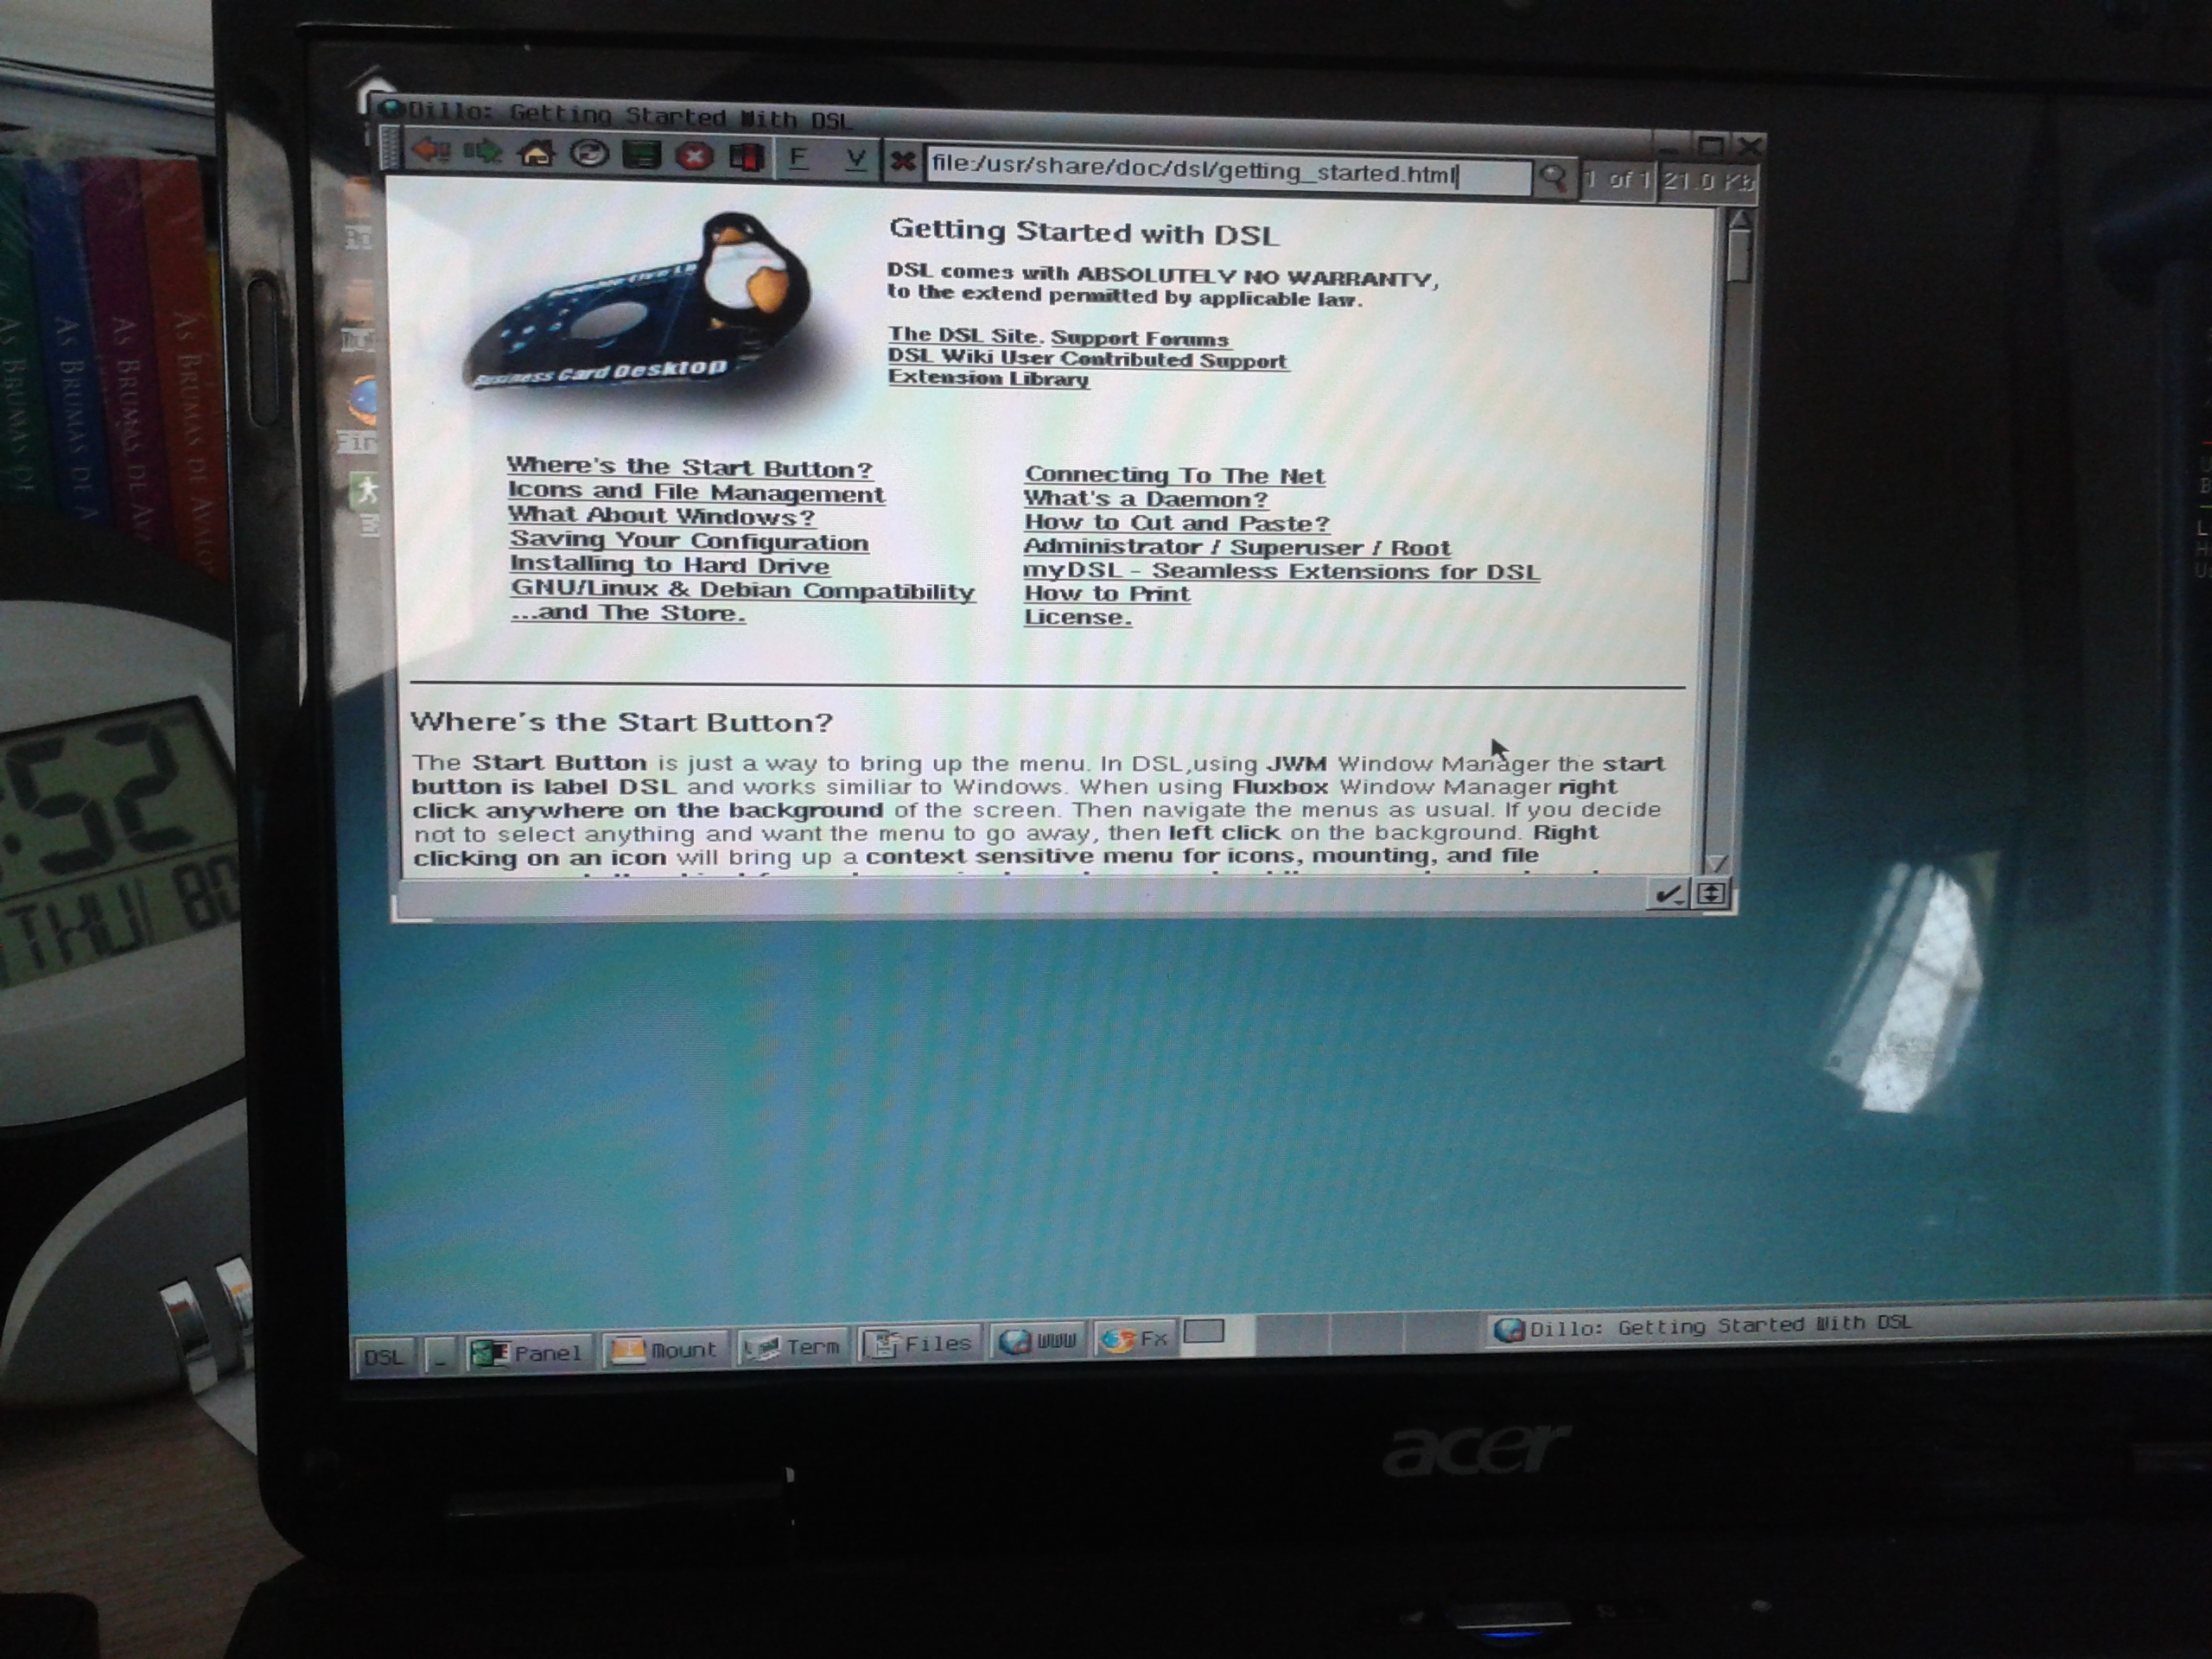
\includegraphics[scale=0.075]{dsl.jpg}}	

	\caption{Damn Small Linux rodando.}

\end{figure}

\section{Conclusão}
A esteganografia digital, ou seja, a arte de esconder
informações em meios digitais, vem sendo cada vez mais pesquisada e utilizada nos dias de hoje. Ela possui uma infinidade de aplicações,
e talvez a mais importante delas seja a segurança da informação, já que, com a esteganografia, as mensagens ficam escondidas nos meios usados,
e a informação passa despercebida por terceiros.
Neste experimento mostrou-se uma técnica simples de esteganografada (LSB), e como ela pode ser utilizada para esconder imagens  dentro de outros
sem comprometer significativamente a qualidade visial das imagens. Em seguida implementou-se uma solução relativamente simples que 
utilizava vários recursos do sistema como : threads, processos (system) e sinais. A esteganografia digital, ou seja, a arte de esconder
informações em meios digitais, vem sendo cada vez mais pesquisada e utilizada nos dias de hoje. Ela possui uma infinidade de aplicações,
e talvez a mais importante delas seja a segurança da informação, já que, com a esteganografia, as mensagens ficam escondidas nos meios usados,
e a informação passa despercebida por terceiros.
%-------------------------------------------------------------------------
\nocite{ex1,ex2}
\bibliographystyle{ieee}
\bibliography{ieee}

\onecolumn
\newpage
\newpage
\section{Anexos}
\subsection{Código do Sistema de decodifica as imagens}
\lstinputlisting[language = C]{exp1.c}
\subsection{Código do processo que adiciona cabeçalho as imagens}
\lstinputlisting[language = C]{cabecalho.c}
\end{document}
  